\documentclass[a4j,titlepage]{jarticle}
\usepackage[dvipdfmx]{graphicx}
\usepackage{url}
\usepackage{here}

%% 本文
\begin{document}

\section{2.現状の課題}
近年、家庭における夫婦の共働きや核家族化の増加(図\ref{fig:1})\cite{bib:tomo}に伴って、保育園などの施設に預けなければならない児童が増えています。しかし、保育園に預けられる児童の数に限りがあるにも関わらず保育園の数や保育士が不足していることで、待機児童の増加が都心部を中心に深刻化しています(図\ref{fig:2}・図\ref{fig:3})\cite{bib:taiki}。待機児童を持つと、母親は出産後の社会復帰が望めない上に、保育園などの教育プログラムを子に受けさせることができないなどの問題があります。また、夫婦の共働きは近所の親同士のつながりが減少する要因にもなり、親の空き時間や親子の時間などといったプライベートのための時間も失われています。「日本のママ白書2017年度版」\cite{bib:mama}の調査では、仲の良いママ友の人数が「0人」と答える人が2014年調査から2017年調査にかけて39.9\%から56.7\%に増えていることが分かっています。

\begin{figure}[H]
\begin{center}
\resizebox{15cm}{!}{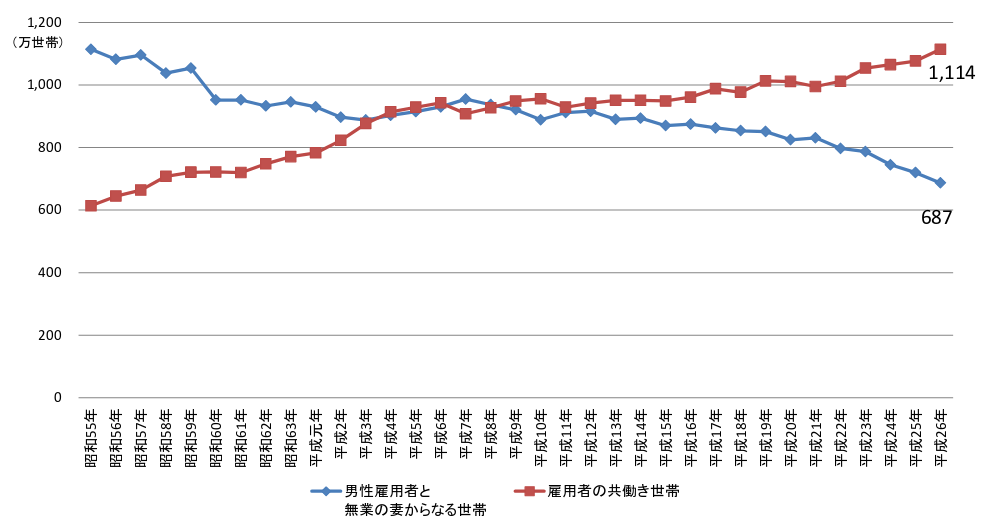
\includegraphics{kadai_v1_document1.png}}
\caption{専業主婦世帯と共働き世帯の推移(厚生労働省調べ)}
\label{fig:1}
\end{center}
\end{figure}

\begin{figure}[H]
\begin{center}
\resizebox{15cm}{!}{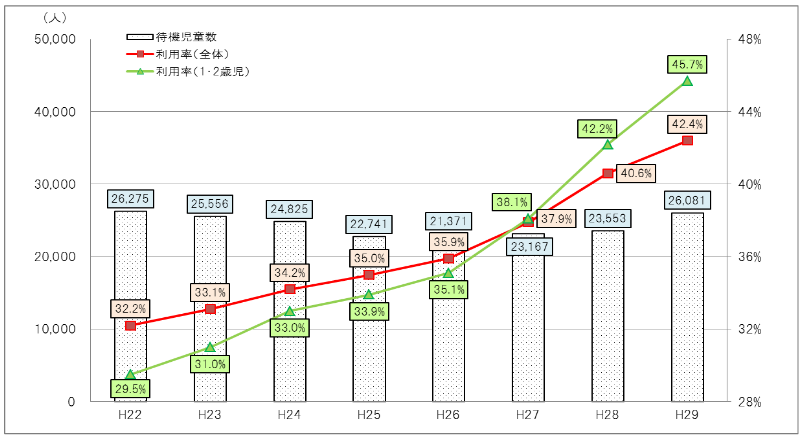
\includegraphics{kadai_v1_document2.png}}
\caption{保育所等待機児童数及び保育所等利用率の推移(厚生労働省調べ)}
\label{fig:2}
\end{center}
\end{figure}

\begin{figure}[H]
\begin{center}
\resizebox{15cm}{!}{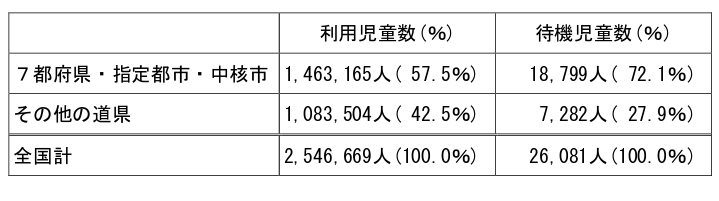
\includegraphics{kadai_v1_document3.png}}
\caption{都市部とそれ以外の地域の待機児童数(厚生労働省調べ)}
\label{fig:3}
\end{center}
\end{figure}

これらの現状から以下のような課題があげられます。

\begin{itemize}
\item 待機児童の教育不足
\item 親同士のつながりの減少
\item 親子及び親自身のプライベートな時間の不足
\end{itemize}

これらの課題を解決するシステムを提案することで、待機児童の教育不足の改善や親同士のつながりの増加、親の空き時間や親子の時間の確保を目指します。

\begin{thebibliography}{3}
\bibitem{bib:tomo}
  専業主婦世帯と共働き世帯の推移.
  \newblock \url{https://www.mhlw.go.jp/file/05-Shingikai-11201000-Roudoukijunkyoku-Soumuka/0000118655.pdf}.
  \newblock 2018年10月11日閲覧.
  
\bibitem{bib:taiki}
  保育所等関連状況取りまとめ(平成29年4月1日).
  \newblock \url{https://www.mhlw.go.jp/file/04-Houdouhappyou-11907000-Koyoukintoujidoukateikyoku-Hoikuka/0000176121.pdf}.
  \newblock 2018年10月11日閲覧.

\bibitem{bib:mama}
  日本のママ白書2017年度版.
  \newblock \url{https://www.mindshare.co.jp/mama/whitepaper2017/}.
  \newblock 2018年10月11日閲覧.  
\end{thebibliography}
\end{document}
